\section{Results of prior-form DWBA calculations}
In a transfer reaction A(d,p)B, the transfer T-matrix has a prior-form formula \cite{thompson2009nuclear}
\begin{equation}\label{eq:priorexact}
T_{\mathrm{prior}}=\langle\Psi_2^{(-)}(\vec{r}_2,\vec{R}_2)\left|V_{nA}(r_n)+U_{pA}(r_p)-U_{dA}(R_1)\right|\phi_{np}\chi_{dA}\rangle,
\end{equation}
where $\phi_{np}$ and $\chi_{dA}$ are bound states wave-functions, $\vec{r}_n=\vec{r}_p+\vec{r}_1$, 
and $U_{dA}(R_1)$ is the auxiliary potential we choose. 
Under first-order DWBA, it becomes
\begin{equation}\label{tprior}
T_{\mathrm{prior}}^{\mathrm{DWBA}}=\langle\phi_{nA}\chi_{pB}^{(-)}\left|V_{nA}(r_n)+U_{pA}(r_p)-U_{dA}(R_1)\right|\phi_{np}\chi_{dA}\rangle,
\end{equation}
\par
The differential cross sections of $^{12}$C(d, p)$^{13}$C calculated in both post and prior forms are given in Fig. \ref{fig:prior}. 
First-order DWBA with finite-range interactions and full complex remnant is used in both calculations. 
The convergence of calculations in prior form is checked in the same way as we discussed in Sec. \ref{sec:post}. 
Variables $rnl$ and $centre$ are chosen based on FRESCO's recommendations. 
As shown in Fig. \ref{fig:prior}, the results from post- and prior-form calculations are close to each other, 
which agrees with the fact that post and prior forms theoretically give the same results in the first-order DWBA. 
\par
It is worth mentioning that the recommended $rnl$, which represents the non-local range, is larger in prior form (12.50 fm) than that in post form (5.6 fm). 
In post form (Eq. \ref{tpost}) $U_{pA}(r_p)$ and $U_{pB}(R_2)$ are close to each other as nuclei A and B are very similar. 
Thus, the operator in Eq. \ref{tpost} is approximately $V_{np}(r_1)$, which has a very short range. 
However, in prior form (Eq. \ref{tprior}) $U_{pA}(r_p)$ and $U_{dA}(R_1)$ cannot cancel each other as the elastic scatterings of deuteron on A and proton on A are very different. 
Thus, the operator in Eq. \ref{tprior} has a longer range which comes from optical potentials $U_{pA}(r_p)$ and $U_{dA}(R_1)$. 
A larger $rnl$ in prior-form calculation also leads to a longer runtime. 
 \begin{figure}[tb]
	\begin{subfigure}{0.5\textwidth}
		\centering
		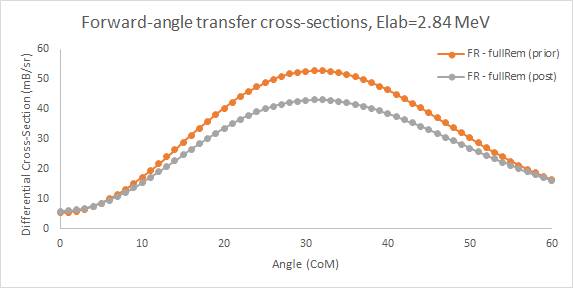
\includegraphics[width=0.98\textwidth]{3MeVReactionsQ5.png}
		\caption{Beam energy is 2.84 MeV. }
		\label{fig:prior-3MeV}
	\end{subfigure}
	\begin{subfigure}{0.5\textwidth}
		\centering
		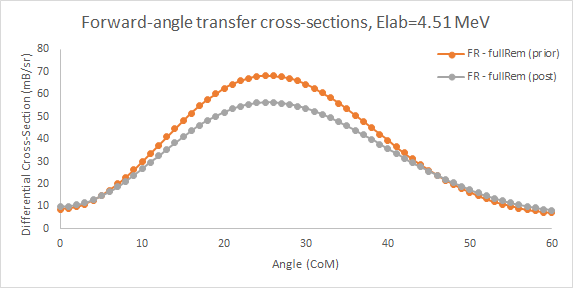
\includegraphics[width=0.98\textwidth]{5MeVReactionsQ5.png}
		\caption{Beam energy is 4.51 MeV. }
		\label{fig:prior-5MeV}
	\end{subfigure}
	\caption{Forward-angled differential cross sections calculated under: 1) first-order DWBA in post form, finite range, with full complex remnant [FR - fullRem (post-form)]; 2) first-order DWBA in prior form, finite range, with full complex remnant [FR - fullRem (prior-form)]. }
%		Left and right panels are for 2.84 MeV and 4.51 MeV repectively.}
	\label{fig:prior}
\end{figure}